\subsection{\label{}Oscillation of the tuning fork}

A tuning fork is an acoustic resonator in the shape of a fork with two prongs, forming a U. it is usually made of elastic metal, as f.i. Steel. Apart from the fundamental mode, as illustrated in \ref{fig:tuning}, the tuning fork can also oscillate in higher overtones. Due to the fact, that these higher modes are damped more strongly by the base, they die out faster and leave a a typical pure musical tone. This also causes the short “clang”, that appears when tipping the fork. The pitch of a particular tuning fork depends on the length as well as on the mass of the prongs.

\begin{figure}[H]
	\centering
	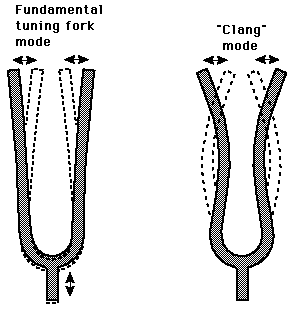
\includegraphics[angle=0,width=0.6\textwidth]{img/tuning}
	\caption{First two balanced modes of a tuning fork.}
	\label{fig:tuning}
\end{figure}

Apart from the modes in which the two prongs oscillate in antiphase, of which the two first are shown in \ref{fig:tuning}, more unbalanced modes exist that transfer onto the base. As the base is in general fixed by holding the tuning fork in the hand or having it fixed by other means, these modes generally don't appear significantly.
The main interest was to measure amplitude and frequency of the vibrations of the tuning fork. To do so, the difference and the sum of the two currents as given out by the electric circuit explained in \ref{} were processed with labview. To calibrate the PSD, the micrometer screw attached to the slide of the tuning fork was used.

In \ref{fig:frequency} the vibration of the tuning fork after 3 seconds of damping is illustrated. The difference of the two currents, that the PSD feeds the electric circuit with, is depicted as a function of the time. As can be seen the tuning fork is harmonically oscillating at a steady frequency.

\begin{figure}[H]
	\centering
	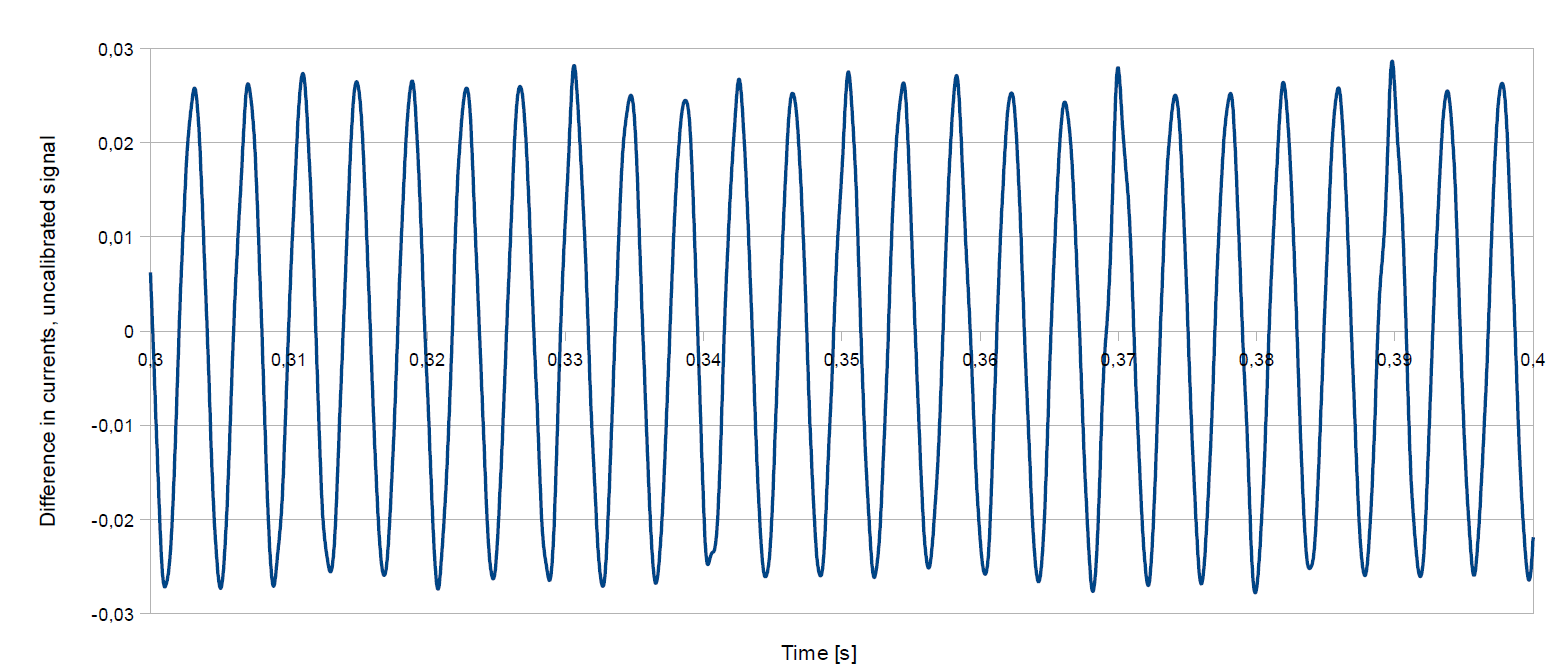
\includegraphics[angle=0,width=0.6\textwidth]{img/frequency}
	\caption{Uncalibrated difference in currents given out by the PSD.}
	\label{fig:frequency}
\end{figure}

This frequency was determined by averaging the periodic time $T$ over 229 periods. Doing this, a frequency of 

\begin{eqnarray}
f = 253,68 Hz
\end{eqnarray}

was found. This gives a relative deviation of $0,9\%$ from the 256 Hz specified by the manufacturer of the tuning fork. Due to the high number of samples a statistic deviation of this magnitude is unlikely.

In \ref{fig:amplitude} the amplitude of the vibration is shown over time. The amplitude was directly calculated from the signal from labview. It can be well seen how after a short phase of transient oscillation withing the first 5 seconds the amplitude decreases very steadily.

\begin{figure}[H]
	\centering
	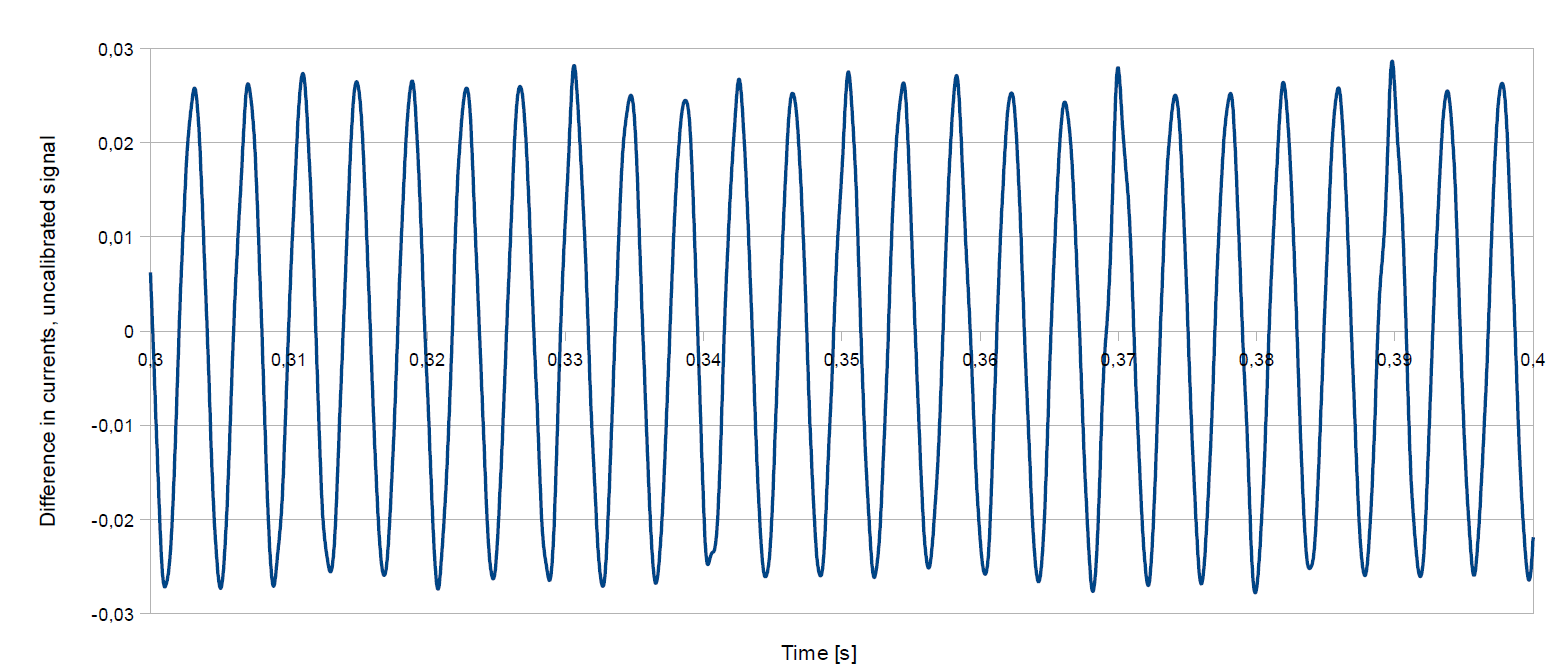
\includegraphics[angle=0,width=0.6\textwidth]{img/frequency}
	\caption{Calibrated amplitude of the oscillations.}
	\label{fig:amplitude}
\end{figure}

Measuring this repeatedly shows that the maximal amplitude highly depends on how hard the tuning fork is stroke, while never exceeding about 0.3 mm and always decreasing in the same way that can me seen in \ref{fig:amplitude}.